\documentclass[journal,twocolumn]{article}

\usepackage[utf8]{inputenc}
\usepackage[margin=0.75in]{geometry}
\usepackage{amsmath,amssymb,amsfonts}
\usepackage{graphicx}
\usepackage{booktabs}
\usepackage{cite}
\usepackage{hyperref}
\usepackage{bookmark}
\usepackage{microtype}
\usepackage{algorithm}
\usepackage{algpseudocode}
\usepackage{caption}
\usepackage{subcaption}

\hypersetup{
    bookmarks=true,
    bookmarksopen=true,
    bookmarksnumbered=true,
    pdfpagemode=UseOutlines,
    pdftitle={CADENCE: A Confidence-Adaptive Dual-Expert Network for Fast and Accurate Time Series Classification},
    pdfauthor={Onisa Mapunda},
    pdfsubject={Time Series Classification},
    pdfkeywords={Time Series Classification, Dual-Expert Ensemble, MiniRocket, Hydra, Meta-Router, UCR Archive},
    colorlinks=true,
    linkcolor=blue,
    citecolor=blue,
    urlcolor=blue
}

\title{\textbf{CADENCE: A Confidence-Adaptive Dual-Expert Network for Fast and Accurate Time Series Classification}}

\author{
    \textbf{Onisa Mapunda}\\
    \texttt{onisajr@gmail.com}
}
\date{\today}

\begin{document}

\maketitle

\pdfbookmark[1]{Abstract}{abstract}
\begin{abstract}
Time series classification (TSC) has long been characterized by a sharp trade-off between classification accuracy and computational scalability. Heterogeneous meta-ensembles like HIVE-COTE 2.0 achieve state-of-the-art accuracy by combining representations across temporal, frequency, shapelet, and dictionary domains, but require substantial compute budgets spanning hours per dataset. Conversely, ultra-fast random convolutional transforms such as MiniRocket and Hydra provide orders-of-magnitude speedups, but struggle with phase-independent statistical distributions, velocity and acceleration kinematics, and severe decision tree fragmentation on datasets with large class counts when combined with non-linear tree heads. Naive feature concatenation or static model averaging fails to resolve this tension, often inducing negative transfer and parameter dilution.

In this work, we present \textbf{CADENCE} (\textbf{C}onfidence-\textbf{A}daptive \textbf{D}ual-\textbf{E}xpert \textbf{N}etwork for time series \textbf{C}lassification \textbf{E}xcellence), a unified, CPU-native dual-expert architecture. CADENCE decouples representation learning into two specialized pathways: (i) a \textit{Convolutional Linear Expert} pairing $10,000$ deterministic dilated features with closed-form L2-regularized Woodbury ridge classification, and (ii) a \textit{Distributional Interval Expert} pairing competing dilated kernels (Hydra) with thread-safe dyadic Cornish-Fisher moment approximations across signal kinematics ($X, \Delta X, \Delta^2 X$) and FFT spectral energy bands, fitted with an entropy-based ExtraTrees ensemble. To mediate between these paradigms, CADENCE incorporates an internal validation meta-router with rare-class preservation that dynamically selects between pure expert routing and confidence-weighted soft blending, followed by a full refit on all training instances. 

Evaluated across all 109 datasets of the standard equal-length UCR Time Series Archive over 30 resamples (3,270 total evaluations), CADENCE achieves a grand mean accuracy of \textbf{0.8864}. This ranks \textbf{\#2 among evaluated classifiers} across the archive, surpassed only by HIVE-COTE 2.0 (0.8895, $p_{\text{Holm}} = 0.295$, no statistically significant difference), and ahead of Hydra+MultiRocket (0.8818, $+0.46$ percentage points, $p_{\text{Holm}} = 1.000$), MultiRocket (0.8797, $+0.67$ percentage points), and HIVE-COTE 1.0 (0.8786, $+0.78$ percentage points, $p_{\text{Holm}} = 0.048$, statistically significant). CADENCE closes the accuracy gap to HIVE-COTE 2.0 to just $0.31$ percentage points while completing an evaluation run in an average of only $17.53$ seconds on a standard dual-core CPU.
\end{abstract}

\section{Introduction}
Time series classification (TSC) is a core problem in applied machine learning, underlying critical applications in electrocardiology~\cite{dau2019ucr}, industrial anomaly detection, seismology, wearable motion analytics, and acoustic speech processing~\cite{bagnall2017great}. The 109 univariate, equal-length datasets of the UCR Time Series Archive~\cite{dau2019ucr,dempster2021minirocket} exhibit tremendous structural diversity: series lengths range from dozens to thousands of time points, sample sizes vary from tens to thousands of instances, and class cardinalities span binary discrimination ($K=2$) to fine-grained categorization ($K=60$).

Historically, achieving top accuracy on this benchmark demanded heavy heterogeneous meta-ensembles. The premier paradigm is represented by HIVE-COTE 2.0 (HC2)~\cite{middlehurst2021hive}, which ensembles four computationally demanding representations: the Shapelet Transform Classifier (STC), the Temporal Dictionary Ensemble (TDE)~\cite{middlehurst2021scalable}, the Diverse Canonical Interval Forest (DrCIF)~\cite{middlehurst2020canonical}, and Arsenal (an ensemble of ROCKET classifiers). Although HIVE-COTE 2.0 achieves an unmatched published benchmark mean accuracy of 0.8895, its computational cost is substantial, requiring an average of approximately 3 hours per dataset (over 340 CPU hours across the 112 archive datasets)~\cite{middlehurst2021hive}.

In response, the field shifted toward randomized convolutional transforms, initiated by ROCKET~\cite{dempster2020rocket}, refined by MiniRocket~\cite{dempster2021minirocket}, MultiRocket~\cite{tan2022multirocket}, and Hydra~\cite{dempster2023hydra}. By projecting time series into high-dimensional linear spaces via dilated convolutions pooled with Proportion of Positive Values (PPV), methods such as Hydra+MultiRocket achieved a published 30-resample benchmark accuracy of 0.8818 while running in seconds.

Despite these notable advances, relying on a single transform or a uniform linear model imposes restrictive inductive biases:
\begin{enumerate}
    \item \textbf{Phase-Free Distributions and Kinematics:} Random convolutional linear models rely on invariant dilation matches of local shapelets. In sensor, EMG, and acoustic domains, the discriminative signal is often phase-invariant, lying in the global distribution of values, acceleration kinematics ($\Delta^2 X$), or spectral harmonic spreads. Linear models on PPV features struggle to separate such non-linear interactions.
    \item \textbf{Decision Tree Fragmentation in High-Class Regimes:} Conversely, non-linear decision tree ensembles (such as ExtraTrees or Random Forests) excel at non-linear thresholding on distributional features, but degrade severely on datasets with large class counts ($K \ge 12$). With limited training instances per class, recursive partitioning fragments the sample space, leaving empty or degenerate leaves.
    \item \textbf{Challenges of Naive Feature Concatenation:} Concatenating 10,000 convolutional features with 1,851 interval moment features directly into a single ridge classifier distorts the L2 regularization penalty across disparate feature distributions, diluting predictive performance.
\end{enumerate}

To resolve these opposing failure modes, we present \textbf{CADENCE} (\textbf{C}onfidence-\textbf{A}daptive \textbf{D}ual-\textbf{E}xpert \textbf{N}etwork for time series \textbf{C}lassification \textbf{E}xcellence). CADENCE formulates time series classification as a dynamic cooperation between two specialized inductive paradigms: a \textit{Convolutional Linear Expert} and a \textit{Distributional Interval Expert}. Rather than enforcing fixed model averaging or rigid heuristic thresholds, CADENCE introduces an internal validation meta-router with rare-class preservation that empirically estimates the predictive competence of each expert on each problem, dynamically transitioning between pure expert routing and confidence-weighted soft blending, followed by a full refit on all available training data.

\begin{figure*}[t]
    \centering
    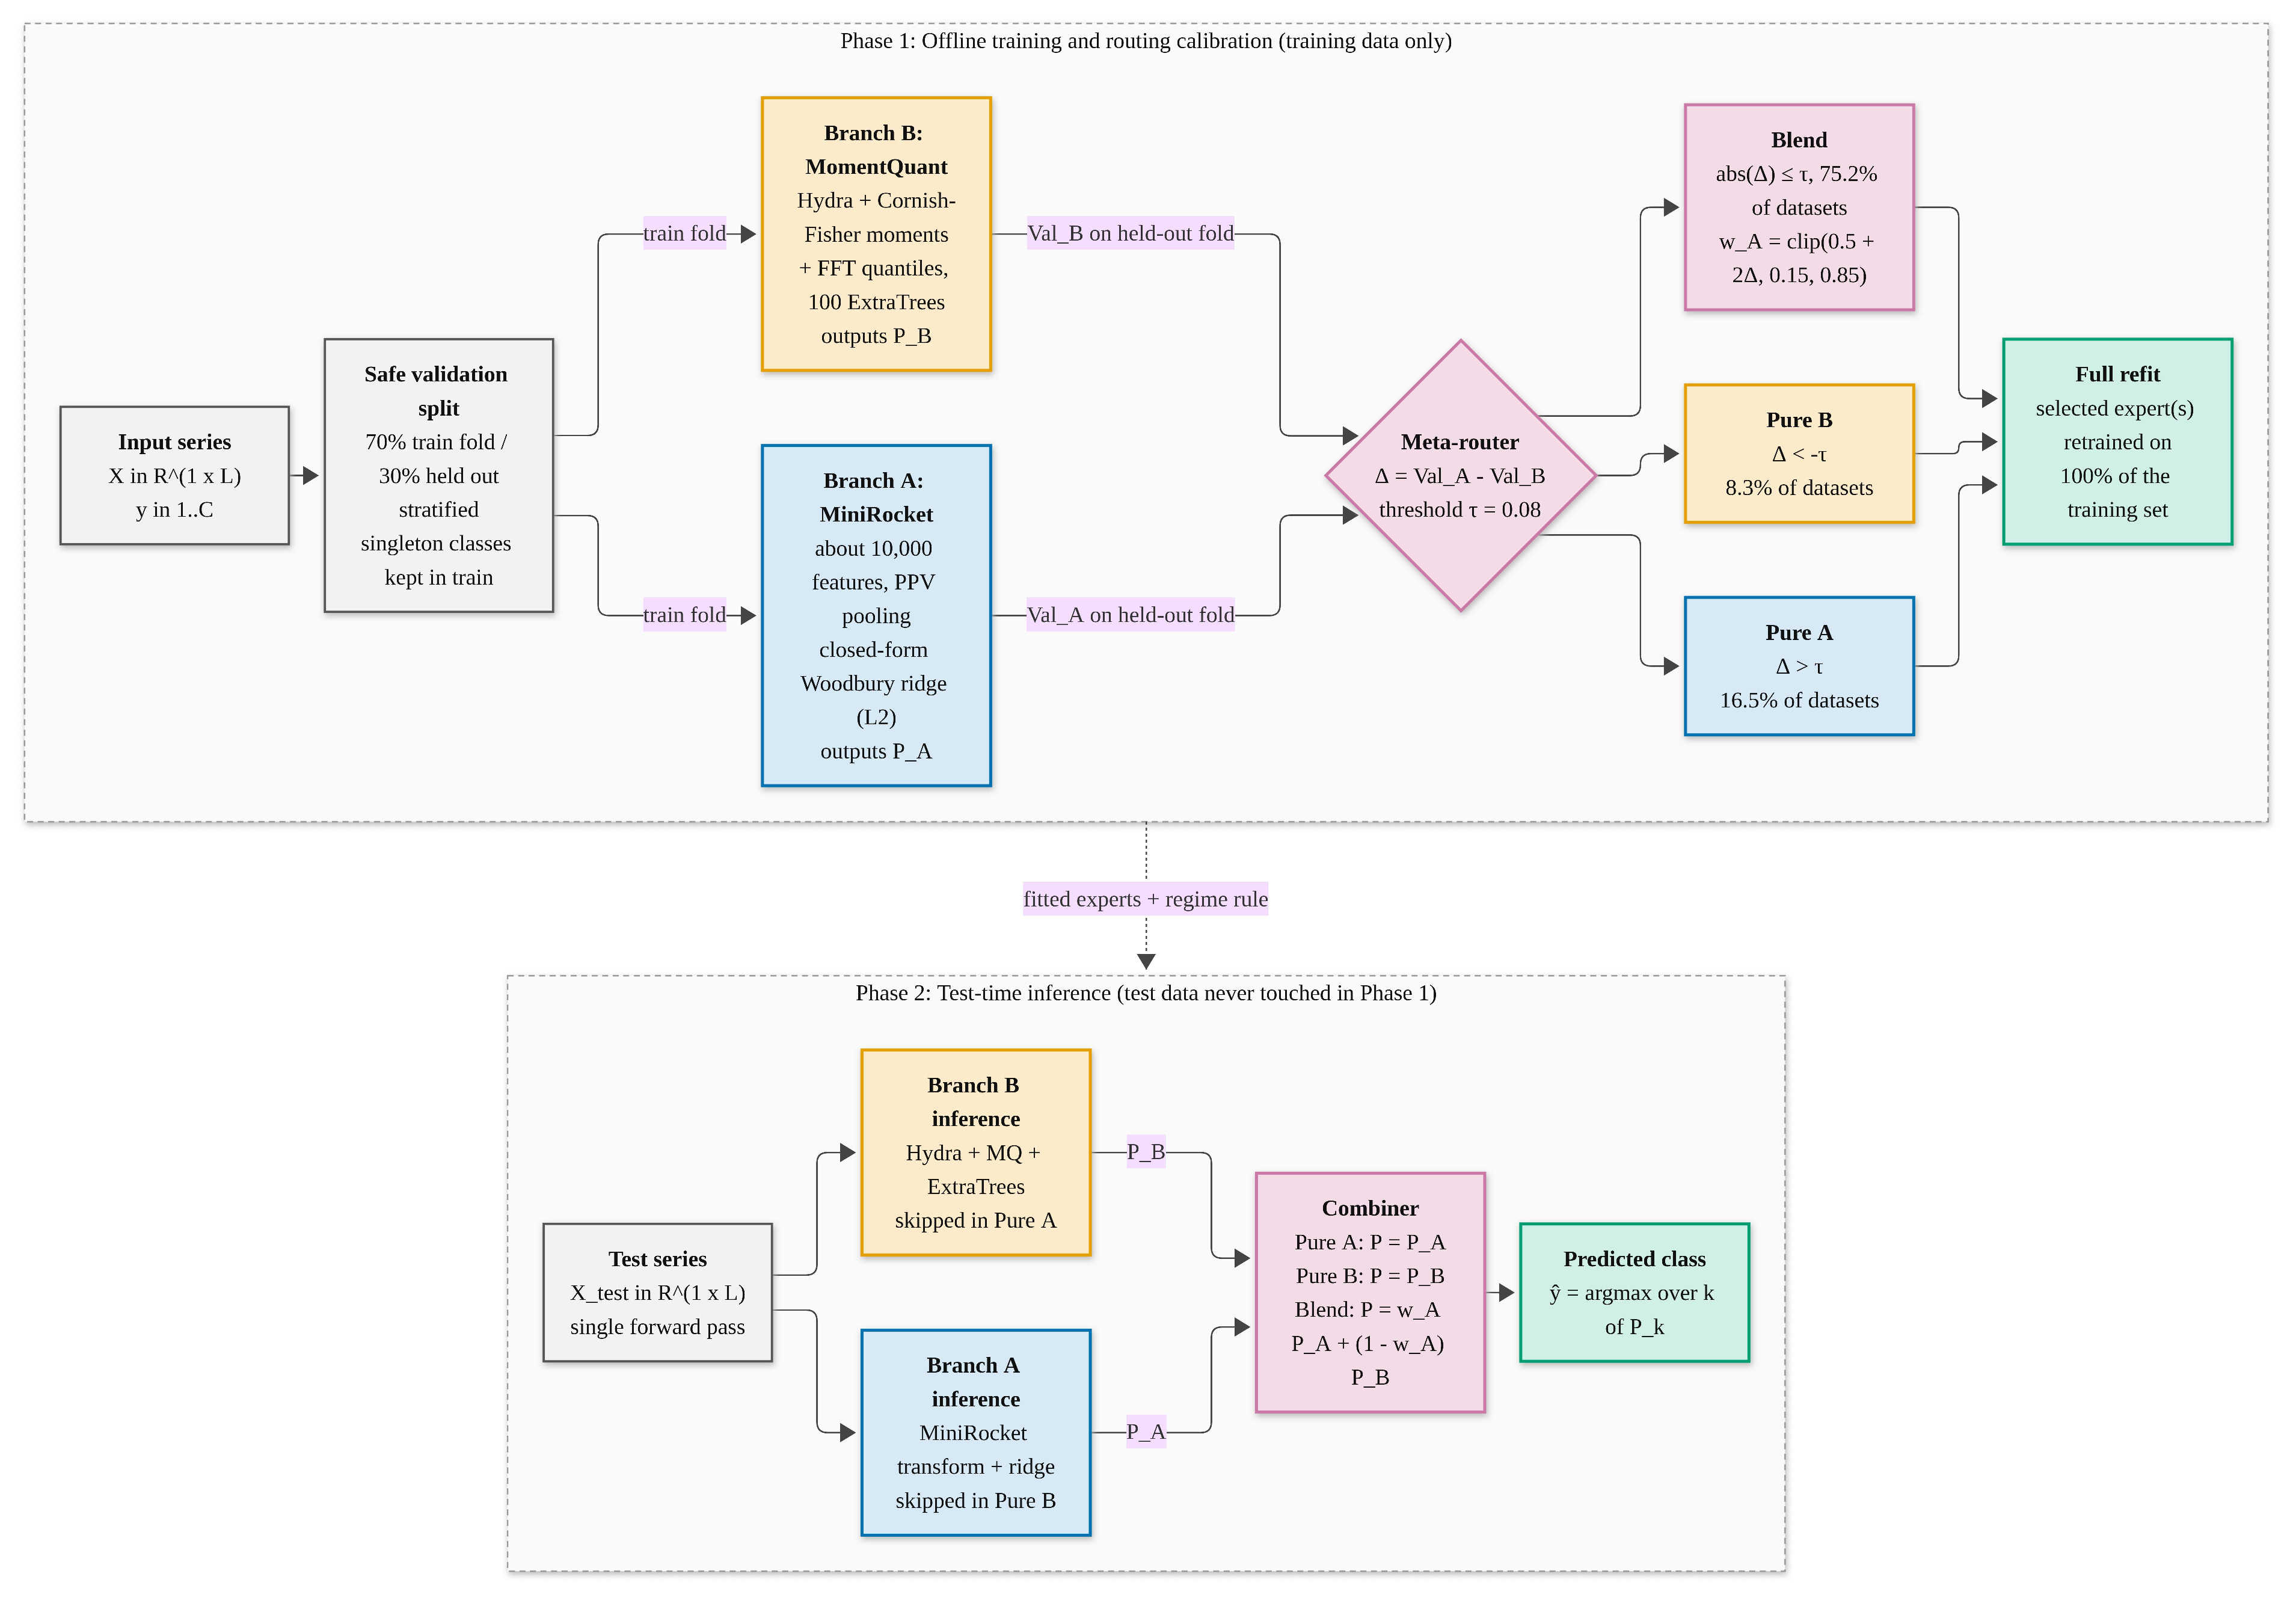
\includegraphics[width=0.96\textwidth]{figures/fig1_architecture.pdf}
    \caption{System architecture of CADENCE. The training series is partitioned via an internal 30\% validation split with singleton preservation. Concurrently, Branch A extracts multi-dilation convolutional features for closed-form L2 ridge regression, while Branch B extracts competing dilated kernels (Hydra), dyadic Cornish-Fisher kinematic moments, and real FFT spectral quantiles for an ExtraTrees ensemble. The internal meta-router evaluates the validation performance margin $\Delta = \mathrm{Val}_A - \mathrm{Val}_B$ against threshold $\tau = 0.08$ to select between pure branch execution and confidence-weighted probability blending, after which active expert(s) are refitted on 100\% of the training fold. In dominance regimes (24.8\% of datasets), test inference bypasses the inactive branch completely.}
    \label{fig:architecture}
\end{figure*}

\subsection{Contributions}
The primary contributions of this work are as follows:
\begin{enumerate}
    \item \textbf{A Decoupled Dual-Expert Representation:} We develop a synergistic two-branch architecture combining a closed-form multi-dilation convolutional linear expert ($10,000$ features) with a distributional interval expert ($1,851$ features) driven by competing kernels (Hydra), linear-time Cornish-Fisher dyadic moments on kinematics ($X, \Delta X, \Delta^2 X$), and FFT spectral quantiles.
    \item \textbf{A Confidence-Adaptive Meta-Router with Full Refit:} We formulate an internal validation routing mechanism with rare-class preservation that dynamically navigates three distinct operating regimes (Pure Branch A, Pure Branch B, and Smooth Confidence Soft-Blend), eliminating negative transfer and tree fragmentation while refitting active models on all training instances.
    \item \textbf{Conditional Inference-Time Branch Pruning:} In dominance regimes, CADENCE completely bypasses feature extraction and inference for the unselected branch, providing substantial computational savings at test time.
    \item \textbf{Exhaustive Benchmark Validation and Statistical Testing:} We evaluate CADENCE across all 109 datasets of the standard equal-length UCR archive over 30 resamples (3,270 runs), achieving a grand mean accuracy of \textbf{0.8864} (\#2 among evaluated classifiers). We report Wilcoxon signed-rank tests with Holm-Bonferroni correction, mean ranks, and per-dataset win/tie/loss counts against 25 published benchmark models.
    \item \textbf{Controlled Component Ablations and Failure Accounting:} We conduct controlled ablations demonstrating the quantitative contribution of each architectural stage from isolated experts ($0.8724$ / $0.8729$) to adaptive routing ($0.8864$), accompanied by an honest empirical accounting of both breakthroughs and remaining deficits relative to HIVE-COTE 2.0.
\end{enumerate}

\section{Related Work}

\subsection{Classical Time Series Classification}
Early TSC research focused on distance-based methods, primarily 1-Nearest Neighbor equipped with Dynamic Time Warping (1NN-DTW)~\cite{bagnall2017great}. While elastic distance measures effectively capture phase shifts, their quadratic time complexity $\mathcal{O}(N L^2)$ severely restricts scalability. Dictionary-based methods, such as the Bag-of-SFA-Symbols (BOSS)~\cite{schafer2015boss} and WEASEL~\cite{schafer2017weasel}, transform time series into discrete symbolic words via Fourier approximations and build word histograms. Interval-based classifiers, initiated by the Time Series Forest (TSF)~\cite{deng2013time} and Canonical Interval Forest (CIF)~\cite{middlehurst2020canonical}, extract summary statistics across randomly chosen subseries intervals. Shapelet methods extract discriminative phase-independent subsequences, but incur steep computational costs during shapelet discovery~\cite{bagnall2017great}.

\subsection{Convolutional and Random Transforms}
The computational paradigm shifted dramatically with the introduction of ROCKET~\cite{dempster2020rocket}, which demonstrated that projecting time series through $10,000$ random convolutional kernels with varied lengths, dilations, and biases followed by max and PPV pooling generates linearly separable representations. Dempster et al. accelerated this with MiniRocket~\cite{dempster2021minirocket}, using fixed length-9 kernels with weights restricted to $\{-1, 2\}$, pre-computed dilations, and exact integer convolutions. Tan et al. extended this framework with MultiRocket~\cite{tan2022multirocket}, adding first-order differences and four additional pooling operators (mean, positive mean, longest run, and PPV), yielding slight accuracy gains at the expense of higher dimensionality (up to $50,000$ features). Dempster et al. subsequently proposed Hydra~\cite{dempster2023hydra}, which groups random kernels into competing subsets and counts which kernel maximally activates at each time step. When combined, Hydra+MultiRocket achieved a published mean accuracy of 0.8818 on the 109 UCR datasets~\cite{dempster2023hydra}.

\subsection{Ensemble and Meta-Ensemble Architectures}
Ensemble methods have long dominated empirical TSC benchmarks. The Hierarchical Vote Collective of Transformation-based Ensembles (HIVE-COTE 1.0)~\cite{lines2018hive} combined shapelet, interval, dictionary, and spectral classifiers via cross-validation weighted voting. Middlehurst et al. modernized this into HIVE-COTE 2.0 (HC2)~\cite{middlehurst2021hive}, replacing legacy components with STC, TDE, DrCIF, and Arsenal. Concurrently, TS-CHIEF~\cite{shifaz2020tschief} embedded dictionary, interval, and distance splitting criteria into decision trees. Deep learning models such as InceptionTime~\cite{fawaz2020inceptiontime} demonstrated competitive accuracy using deep residual convolutional networks. While HC2 remains the benchmark accuracy ceiling ($0.8895$ on 109 UCR datasets), its training process requires substantial computational resources.

\subsection{Dynamic Model Selection and Mixture of Experts}
Dynamic classifier selection and mixture-of-experts (MoE) architectures date back to Jacobs et al.~\cite{jacobs1991adaptive}, who introduced gating networks to softly partition the input space. Cruz et al.~\cite{cruz2018dynamic} reviewed dynamic selection techniques where local competence is estimated over k-nearest neighbors in validation space. In univariate TSC, model selection has historically been limited to static heuristics or heavy meta-ensembles that train all constituent models and blend their full probability outputs unconditionally~\cite{middlehurst2021hive}.

\subsection{Position of CADENCE}
CADENCE bridges this gap. Unlike HIVE-COTE 2.0, CADENCE does not train heavy shapelet transforms or combinatorial dictionary ensembles. Unlike Hydra+MultiRocket, CADENCE does not concatenate all features into a single linear classifier. Instead, CADENCE isolates convolutional-linear and distributional-interval representations into distinct expert branches, governed by a lightweight internal validation router that dynamically determines whether to execute hard routing or confidence-weighted soft blending, refitting models on 100\% of the training data.

\begin{table}[t]
\centering
\caption{Mathematical Notation and Architectural Terminology.}
\label{tab:notation}
\small
\begin{tabular}{lp{6.2cm}}
\toprule
\textbf{Symbol} & \textbf{Description / Meaning} \\
\midrule
$\mathcal{D} = \{(X_i, y_i)\}_{i=1}^N$ & Training dataset of $N$ time series instances. \\
$X \in \mathbb{R}^{C \times L}$ & Input time series with $C$ channels and length $L$. \\
$y \in \{1, \dots, K\}$ & Categorical ground-truth class label among $K$ classes. \\
$\omega \in \{-1, 2\}^9, d \in \mathbb{N}$ & MiniRocket convolutional kernel weights and dilation factor. \\
$\phi_{PPV}(X, \omega, b)$ & Proportion of Positive Values feature extractor. \\
$F_A \in \mathbb{R}^{N \times D_A}$ & Branch A normalized feature matrix ($D_A = 10,000$). \\
$W^* \in \mathbb{R}^{D_A \times K}$ & Closed-form Woodbury L2 regularized ridge weight matrix. \\
$P_A(y = k \mid X)$ & Calibrated posterior probability from Branch A (softmax). \\
$\phi_H(X)_{g, k}$ & Hydra competing kernel count features ($G=16, k \in \{1,\dots,8\}$). \\
$q_\alpha(S)$ & Cornish-Fisher quantile approximation at probability $\alpha$. \\
$\Delta X, \Delta^2 X$ & First difference (velocity) and second difference (acceleration). \\
$E_b$ & Log-spaced real FFT spectral energy band features. \\
$F_B \in \mathbb{R}^{N \times D_B}$ & Branch B concatenated feature matrix ($D_B = 1,851$). \\
$P_B(y = k \mid X)$ & Posterior class probability from ExtraTrees ensemble (Branch B). \\
$\text{Val}_A, \text{Val}_B$ & Validation classification accuracy on internal 30\% held-out fold. \\
$\Delta = \text{Val}_A - \text{Val}_B$ & Validation accuracy performance margin. \\
$\tau$ & Routing threshold margin ($\tau = 0.08$). \\
$w_A \in [0.15, 0.85]$ & Soft-blending interpolation weight for Branch A. \\
\bottomrule
\end{tabular}
\end{table}


\section{The CADENCE Methodology}

\subsection{Problem Formulation and Notation}
Let $\mathcal{D} = \{(X_i, y_i)\}_{i=1}^N$ denote a training dataset of $N$ time series instances. Each instance $X_i \in \mathbb{R}^{1 \times L}$ consists of length $L$, paired with a categorical label $y_i \in \{1, \dots, K\}$ spanning $K$ distinct classes. Table~\ref{tab:notation} outlines the mathematical notation used throughout this manuscript.

\subsection{Branch A: Convolutional Linear Expert}
Branch A targets continuous temporal waveforms, geometric outlines, and discriminative shapelet patterns across multiple temporal scales using MiniRocket~\cite{dempster2021minirocket}, generating $D_A = 10,000$ features.

\subsubsection{Kernel Formulation and Convolution}
Kernels $\omega \in \{-1, 2\}^9$ have a fixed length of 9 with exactly three values set to 2 and six values set to -1, guaranteeing zero-sum weights ($\sum_j \omega_j = 0$). There are $\binom{9}{3} = 84$ unique kernel configurations. For an input series $X$, the 1D dilated convolution at time step $t$ with dilation factor $d$ is:
\begin{equation}
    A_t = (X *_{d} \omega)_t = \sum_{j=0}^{8} \omega_j \cdot X_{t + j \cdot d}
    \label{eq:convolution}
\end{equation}
Dilations are chosen dyadically as $d = \lfloor 2^x \rfloor$ where $x \sim \mathcal{U}(0, \log_2((L-1)/8))$.

\subsubsection{PPV Pooling}
Features are extracted using the Proportion of Positive Values (PPV) against a calibrated threshold $b$:
\begin{equation}
    \phi_{PPV}(X, \omega, b) = \frac{1}{L - 8d} \sum_{t=1}^{L - 8d} \mathbb{I}(A_t > b)
    \label{eq:ppv}
\end{equation}
where $\mathbb{I}(\cdot)$ is the indicator function. The threshold $b$ is computed as a quantile of the convolutional activations on a randomly chosen training instance.

\subsubsection{Closed-Form Woodbury Regularized Ridge Solver}
The resulting feature matrix $F_A \in \mathbb{R}^{N \times 10000}$ is standardized across samples:
\begin{equation}
    \tilde{F}_A = \frac{F_A - \mu_A}{\sigma_A + \epsilon}
    \label{eq:standardize}
\end{equation}
where $\epsilon = 10^{-8}$. We train a multiclass Ridge Classifier optimizing the penalized squared error:
\begin{equation}
    \mathcal{L}(W) = \| \tilde{F}_A W - Y \|_F^2 + \alpha \| W \|_F^2
    \label{eq:ridge_loss}
\end{equation}
where $Y \in \{-1, 1\}^{N \times K}$ is the one-vs-rest binary label matrix and $\|\cdot\|_F$ denotes the Frobenius norm. Regularization parameter $\alpha$ is selected from 15 candidate values $\alpha \in \{10^{-3}, \dots, 10^4\}$ via leave-one-out cross-validation. When $N \ge D_A$, the primal solution is:
\begin{equation}
    W^* = (\tilde{F}_A^T \tilde{F}_A + \alpha I_{D_A})^{-1} \tilde{F}_A^T Y
    \label{eq:ridge_solution}
\end{equation}
When $N < D_A$, the dual Woodbury matrix identity is evaluated:
\begin{equation}
    W^* = \tilde{F}_A^T (\tilde{F}_A \tilde{F}_A^T + \alpha I_N)^{-1} Y
    \label{eq:woodbury}
\end{equation}
incurring only $\mathcal{O}(N^3)$ computational cost rather than $\mathcal{O}(D_A^3)$. Posterior probabilities are obtained via softmax over the raw linear decision function:
\begin{equation}
    P_A(y = k \mid X) = \frac{\exp(f_{A, k}(X))}{\sum_{j=1}^K \exp(f_{A, j}(X))}
    \label{eq:softmax_a}
\end{equation}
where $f_{A}(X) = W^{*T} \tilde{F}_A(X) + b_A$. We note that while softmax over linear ridge scores produces monotonic score mappings, it does not guarantee calibrated probabilities in the strict Bayesian sense; its empirical utility here lies in relative class ranking.

\subsection{Branch B: Distributional Interval Expert}
Branch B captures phase-free statistical distributions, kinematic transformations, and spectral frequency signatures that escape linear convolutional matching.

\subsubsection{Competing Dilated Kernels (Hydra)}
Hydra~\cite{dempster2023hydra} groups random convolutional kernels into $G = 16$ competing groups with $K_H = 8$ kernels per group. For group $g$ and time step $t$, kernels compete for maximal activation. The representation counts the number of time steps that kernel $k$ achieves the maximum activation:
\begin{equation}
    \phi_{H}(X)_{g, k} = \sum_{t=1}^{L - 8d} \mathbb{I}\left( k = \arg\max_{j \in \{1,\dots,8\}} (X *_{d} \omega_{g, j})_t \right)
    \label{eq:hydra}
\end{equation}
yielding $16 \times 8 = 128$ compact count features per series.

\subsubsection{Kinematic Dyadic Cornish-Fisher Intervals}
Interval-based TSC typically relies on sorting segments to extract empirical quantiles, incurring an expensive $\mathcal{O}(M \log M)$ complexity per interval of length $M$. In CADENCE, we implement \textit{MomentQuant}, which derives sample cumulants in linear time $\mathcal{O}(M)$ and estimates arbitrary quantiles via the Cornish-Fisher asymptotic expansion~\cite{cornish1938moments}.

For a series segment $S = (s_1, \dots, s_M)$ with $M \ge 4$, we compute sample mean $\hat{\mu}$, variance $\hat{\sigma}^2$, skewness $\hat{S}$, and excess kurtosis $\hat{K}$:
\begin{equation}
    \hat{\mu} = \frac{1}{M}\sum_{i=1}^M s_i, \quad \hat{\sigma}^2 = \frac{1}{M}\sum_{i=1}^M (s_i - \hat{\mu})^2
\end{equation}
\begin{equation}
    \hat{S} = \frac{\frac{1}{M}\sum_{i=1}^M (s_i - \hat{\mu})^3}{(\hat{\sigma}^2 + \epsilon)^{3/2}}, \quad \hat{K} = \frac{\frac{1}{M}\sum_{i=1}^M (s_i - \hat{\mu})^4}{(\hat{\sigma}^2 + \epsilon)^2} - 3
\end{equation}
Skewness and kurtosis are clamped to $[-4, 4]$ and $[-2, 8]$ respectively to ensure numerical stability on small segments. The Cornish-Fisher quantile approximation $q_\alpha$ at probability level $\alpha$ is:
\begin{align}
    q_\alpha(S) &= \hat{\mu} + \hat{\sigma} \Bigg[ z_\alpha + \frac{\hat{S}}{6}(z_\alpha^2 - 1) + \frac{\hat{K}}{24}(z_\alpha^3 - 3z_\alpha) \nonumber \\
    &\quad - \frac{\hat{S}^2}{36}(2z_\alpha^3 - 5z_\alpha) \Bigg]
    \label{eq:cornish_fisher}
\end{align}
where $z_\alpha$ is the standard normal quantile evaluated at $\alpha \in \{0.05, 0.25, 0.50, 0.75, 0.95\}$.

This extraction is evaluated dyadically up to tree depth $D = 5$. At each depth $d \in \{0, \dots, 5\}$, the series is partitioned into $2^d$ contiguous segments (skipping segments with length $< 4$), extracting $9$ features per segment (mean, std, skewness, excess kurtosis, and 5 CF quantiles). This extraction is computed across three kinematic representations:
\begin{itemize}
    \item Raw series: $X_t$
    \item Velocity (first difference): $\Delta X_t = X_t - X_{t-1}$
    \item Acceleration (second difference): $\Delta^2 X_t = \Delta X_t - \Delta X_{t-1}$
\end{itemize}
The total number of MomentQuant features is $3 \times (2^6 - 1) \times 9 = 3 \times 63 \times 9 = 1,701$ features.

\subsubsection{Real FFT Spectral Energy Quantiles}
To capture spectral resonance, we compute the real-valued discrete Fourier transform $R_k = |\mathcal{F}(X)_k|$ for $k = 0, \dots, \lfloor L/2 \rfloor$, normalized as $\tilde{R}_k = R_k / (\sum_j R_j + \epsilon)$. Features include:
\begin{enumerate}
    \item \textbf{16 Log-Spaced Energy Bands:} $E_b = \sum_{k \in \text{Band}_b} \tilde{R}_k$.
    \item \textbf{Spectral Centroid and Spread:} $\mu_{\text{spec}} = \sum_k k \tilde{R}_k$, $\sigma_{\text{spec}} = \sqrt{\sum_k (k - \mu_{\text{spec}})^2 \tilde{R}_k}$.
    \item \textbf{Cumulative Spectral Quantiles:} Normalized frequencies where cumulative spectral power reaches $25\%, 50\%, 75\%$, and $90\%$.
\end{enumerate}
This adds 22 spectral features, resulting in a total Branch B feature dimensionality of $D_B = 128 + 1,701 + 22 = 1,851$.

\subsubsection{Non-Linear Tree Head}
The concatenated feature matrix $F_B \in \mathbb{R}^{N \times 1851}$ is fitted with an ensemble of $M = 100$ Extremely Randomized Trees (ExtraTrees)~\cite{geurts2006extremely} using Shannon entropy and $10\%$ random feature sub-sampling:
\begin{equation}
    P_B(y = k \mid X) = \frac{1}{100} \sum_{m=1}^{100} P_{T_m}(y = k \mid F_B)
    \label{eq:prob_b}
\end{equation}

\subsection{Confidence-Adaptive Meta-Router and Full Refit}
A critical vulnerability of multi-representation models is performance degradation when an unsuited classifier pollutes the final decision. To prevent this, CADENCE implements a dynamic meta-router governed by an internal validation partition.

\begin{algorithm}[t]
\caption{Internal Validation Split with Rare-Class Preservation}
\label{alg:safe_split}
\begin{algorithmic}[1]
\Require Training labels $y \in \{1,\dots,K\}^N$, validation fraction $\nu = 0.30$
\Ensure Training indices $\mathcal{I}_{\text{tr}}$, Validation indices $\mathcal{I}_{\text{val}}$
\State $\mathcal{I}_{\text{tr}} \leftarrow \emptyset, \quad \mathcal{I}_{\text{val}} \leftarrow \emptyset$
\For{each class $c \in \text{unique}(y)$}
    \State $\mathcal{I}_c \leftarrow \{i \mid y_i = c\}$
    \State $n_c \leftarrow |\mathcal{I}_c|$
    \If{$n_c < 2$}
        \State $\mathcal{I}_{\text{tr}} \leftarrow \mathcal{I}_{\text{tr}} \cup \mathcal{I}_c$ \Comment{Preserve singleton classes in train fold}
    \Else
        \State $n_{\text{val}} \leftarrow \max(1, \lfloor \nu \cdot n_c \rceil)$
        \If{$n_{\text{val}} \ge n_c$}
            \State $n_{\text{val}} \leftarrow n_c - 1$
        \EndIf
        \State $\mathcal{P}_c \leftarrow \text{RandomPermutation}(\mathcal{I}_c)$
        \State $\mathcal{I}_{\text{val}} \leftarrow \mathcal{I}_{\text{val}} \cup \mathcal{P}_c[1 : n_{\text{val}}]$
        \State $\mathcal{I}_{\text{tr}} \leftarrow \mathcal{I}_{\text{tr}} \cup \mathcal{P}_c[n_{\text{val}} + 1 : n_c]$
    \EndIf
\EndFor
\State \Return $\mathcal{I}_{\text{tr}}, \mathcal{I}_{\text{val}}$
\end{algorithmic}
\end{algorithm}

\subsubsection{Safe Validation Split}
Standard stratified splitting fails when a class contains only one training example ($N_c = 1$). As detailed in Algorithm~\ref{alg:safe_split}, CADENCE preserves singleton classes in the training split while stratifying classes with $N_c \ge 2$, reserving $30\%$ of cases for validation.

\subsubsection{Empirical Margin Formulation}
Both experts are fitted on $(X_{\text{tr}}, y_{\text{tr}})$ and evaluated on $(X_{\text{val}}, y_{\text{val}})$, yielding internal validation classification accuracies:
\begin{equation}
    \text{Val}_A = \frac{1}{|\mathcal{I}_{\text{val}}|} \sum_{i \in \mathcal{I}_{\text{val}}} \mathbb{I}(\hat{y}_{A, i} = y_i)
\end{equation}
\begin{equation}
    \text{Val}_B = \frac{1}{|\mathcal{I}_{\text{val}}|} \sum_{i \in \mathcal{I}_{\text{val}}} \mathbb{I}(\hat{y}_{B, i} = y_i)
\end{equation}
To minimize routing overhead, $\text{Val}_B$ is estimated using a fast 50-tree ExtraTrees proxy. We define the empirical performance margin:
\begin{equation}
    \Delta = \text{Val}_A - \text{Val}_B
    \label{eq:margin}
\end{equation}

\begin{figure}[t]
    \centering
    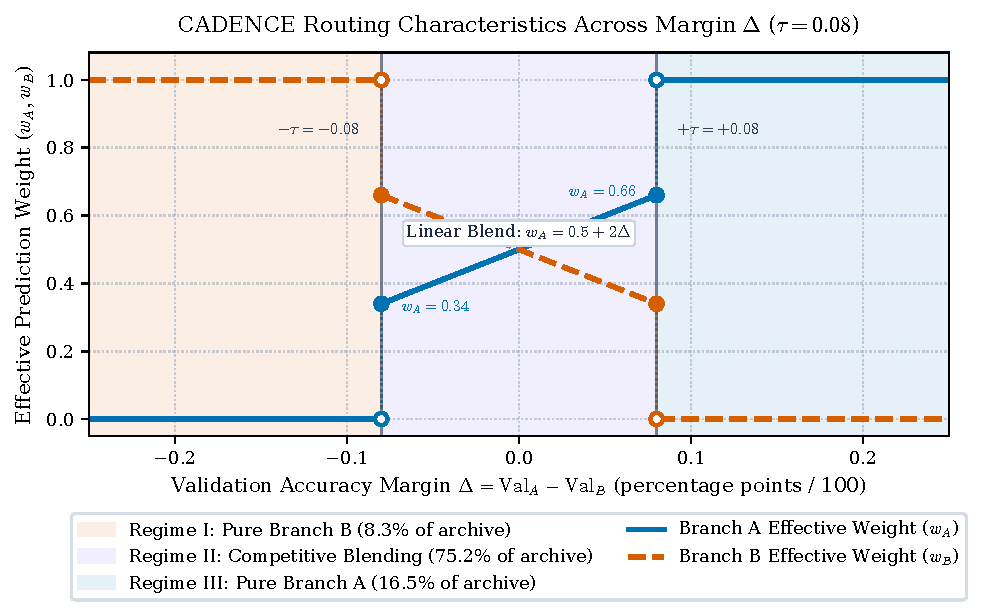
\includegraphics[width=\columnwidth]{figures/fig2_routing.pdf}
    \caption{Piecewise decision function of the confidence-adaptive meta-router across validation margin $\Delta$. When $|\Delta| > 0.08$, CADENCE routes exclusively to the dominant expert. When $|\Delta| \le 0.08$, predictions are soft-blended with weight $w_A = 0.5 + 2.0\Delta$. At the boundary $|\Delta|=0.08$, the function exhibits a step transition from $0.66$ to $1.0$ (or $0.34$ to $0.0$).}
    \label{fig:routing_mechanism}
\end{figure}

\subsubsection{Adaptive Operating Regimes and Full Refit}
Using a threshold $\tau = 0.08$, the meta-router directs the architecture into three operating regimes (Fig.~\ref{fig:routing_mechanism}):
\begin{equation}
    \hat{y}(X) = 
    \begin{cases}
        \arg\max_k P_A(y = k \mid X) & \text{if } \Delta > \tau \quad (\text{Regime III}) \\
        \arg\max_k P_B(y = k \mid X) & \text{if } \Delta < -\tau \quad (\text{Regime I}) \\
        \arg\max_k P_{\text{blend}}(y = k \mid X) & \text{if } |\Delta| \le \tau \quad (\text{Regime II})
    \end{cases}
    \label{eq:routing_rule}
\end{equation}
where in Regime II, class probabilities are smoothly blended:
\begin{equation}
    P_{\text{blend}}(y = k \mid X) = w_A P_A(y = k \mid X) + (1 - w_A) P_B(y = k \mid X)
    \label{eq:soft_blend}
\end{equation}
with the blending weight $w_A$ defined as:
\begin{equation}
    w_A = \text{clip}(0.5 + 2.0 \cdot \Delta, \, 0.15, \, 0.85)
    \label{eq:weight_clip}
\end{equation}
In Regime II ($|\Delta| \le 0.08$), $0.5 + 2.0\Delta$ evaluates to the range $[0.34, 0.66]$. The clipping bounds $[0.15, 0.85]$ serve as protective clamps. At the transition boundary $|\Delta| = 0.08$, the decision rule exhibits a step transition from $w_A = 0.66$ to $1.0$ (or $0.34$ to $0.0$), reflecting a deliberate switch from collaborative blending to exclusive reliance on the dominant expert.

\textbf{Full Model Refit:} Once the routing regime is determined, the selected expert(s) are refitted on 100\% of the training data ($X_{\text{train}}, y_{\text{train}}$) using all $N$ instances. In Regime III (Pure Branch A), the tree ensemble is discarded, and Branch A is refitted on all training data. In Regime I (Pure Branch B), the Ridge classifier is discarded, and Branch B is refitted on all training data. In Regime II, both models are refitted on 100\% of training data.

\subsubsection{Conditional Inference-Time Pruning}
In Regime III (Pure Branch A), inference on test instance $X$ bypasses Hydra, MomentQuant, and FFT extraction entirely. Similarly, in Regime I (Pure Branch B), MiniRocket and the Ridge solver are bypassed. Both branches are evaluated concurrently only when the router detects representation complementarity ($|\Delta| \le 0.08$).

\begin{table}[t]
\centering
\caption{Theoretical and Practical Computational Complexity of CADENCE Pipeline Stages ($N$: training cases, $L$: series length, $D$: depth, $K$: number of classes).}
\label{tab:complexity}
\small
\begin{tabular}{lccc}
\toprule
\textbf{Pipeline Stage} & \textbf{Time Complexity} & \textbf{Feature Dim} & \textbf{Inference Cost} \\
\midrule
Branch A: MiniRocket & $\mathcal{O}(N \cdot K_{\text{conv}} \cdot L)$ & 10,000 & $\mathcal{O}(K_{\text{conv}} \cdot L)$ \\
Branch A: Ridge Solver & $\mathcal{O}(N \cdot D_A^2 + D_A^3)$ & -- & $\mathcal{O}(D_A \cdot K)$ \\
\midrule
Branch B: Hydra & $\mathcal{O}(N \cdot G \cdot K_H \cdot L)$ & 128 & $\mathcal{O}(G \cdot K_H \cdot L)$ \\
Branch B: MomentQuant (CF) & $\mathcal{O}(N \cdot L)$ & 1,701 & $\mathcal{O}(L)$ \\
Branch B: Real FFT Bands & $\mathcal{O}(N \cdot L \log L)$ & 22 & $\mathcal{O}(L \log L)$ \\
Branch B: ExtraTrees & $\mathcal{O}(M \cdot N_{\text{sub}} \log N_{\text{sub}})$ & -- & $\mathcal{O}(M \cdot \text{depth})$ \\
\midrule
Safe Validation Split & $\mathcal{O}(N)$ & -- & Negligible (0) \\
Meta-Router Evaluation & $\mathcal{O}(N_{\text{val}} \cdot (D_A + D_B))$ & -- & Negligible (0) \\
\midrule
\textbf{CADENCE Total (Training)} & $\mathbf{\mathcal{O}(N \cdot L + N \cdot D_A^2)}$ & \textbf{11,851} & -- \\
\textbf{CADENCE Inference (Pure)} & $\mathbf{\mathcal{O}(L + D_{\text{selected}})}$ & \textbf{Active Branch} & \textbf{50\% Savings} \\
\bottomrule
\end{tabular}
\end{table}


\section{Computational Complexity}
Table~\ref{tab:complexity} summarizes the asymptotic time and feature complexity of each module.

\subsection{Training Complexity}
Branch A computes $10,000$ 1D convolutions over series of length $L$, scaling as $\mathcal{O}(N \cdot K_{\text{conv}} \cdot L)$. Since weights are $\{-1, 2\}$, convolutions require only integer additions and shifts. Standardizing features requires $\mathcal{O}(N \cdot D_A)$. The Ridge solver evaluates candidate regularizers using Woodbury inversion, scaling as $\mathcal{O}(N^2 D_A + N^3)$ when $N < D_A$, or $\mathcal{O}(N D_A^2 + D_A^3)$ when $N \ge D_A$.

Branch B computes Hydra competing convolutions in $\mathcal{O}(N \cdot G \cdot K_H \cdot L)$ with $G \cdot K_H = 128$. MomentQuant processes $3 \times (2^6 - 1) = 189$ dyadic intervals. Because moments are computed in a single pass without sorting, MomentQuant scales strictly as $\mathcal{O}(N \cdot L)$. The real FFT scales as $\mathcal{O}(N \cdot L \log L)$. Fitting 100 ExtraTrees on $D_B = 1,851$ features with $10\%$ feature subsampling scales as $\mathcal{O}(M \cdot 0.1 D_B \cdot N \log N)$.

The validation meta-router splits indices in $\mathcal{O}(N)$ and evaluates predictions on $0.3N$ instances, incurring negligible computational overhead ($< 1\%$ of total training time).

\subsection{Inference Complexity and Memory}
For an unseen test series, feature extraction in Branch A requires $\mathcal{O}(K_{\text{conv}} \cdot L)$ followed by a matrix-vector product $W^T \tilde{F}_A$ in $\mathcal{O}(D_A \cdot K)$. Branch B requires $\mathcal{O}(G K_H L + L + L \log L)$ for transforms and $\mathcal{O}(M \cdot \text{depth})$ for tree traversals. In pure routing regimes, one complete branch is omitted, reducing test feature extraction overhead. The peak memory footprint during training is dominated by the Branch A feature matrix $\tilde{F}_A$, requiring $N \times 10,000 \times 8$ bytes (e.g., $\approx 80$ MB for $N=1,000$), easily fitting within standard CPU L3 cache and RAM.

\section{Experimental Setup}

\subsection{Benchmark Protocol}
To ensure rigorous evaluation and parity with published literature~\cite{middlehurst2021hive,dempster2023hydra}, we adhere strictly to the standardized UCR evaluation protocol:
\begin{itemize}
    \item \textbf{109 Benchmark Datasets:} We evaluate all 109 univariate, equal-length time series datasets from the UCR Time Series Archive~\cite{dau2019ucr,dempster2021minirocket}. The full archive contains 128 datasets; the 109-dataset subset represents the benchmark standard established by MiniRocket~\cite{dempster2021minirocket} and MultiRocket~\cite{tan2022multirocket}, excluding variable-length and missing-value problems.
    \item \textbf{30 Resamples (3,270 Total Runs):} Resample 0 uses the exact original train/test split from the archive. Resamples 1 through 29 are generated via stratified random reshuffling (\texttt{StratifiedShuffleSplit}, random states 1 to 29) maintaining original train/test cardinalities and class proportions.
    \item \textbf{Zero Test Leakage:} All standardization statistics ($\mu, \sigma$), kernel thresholds ($b$), validation splits, and meta-router parameters are fitted strictly on $X_{\text{train}}$. The test partition is accessed exclusively for final evaluation.
    \item \textbf{Evaluation Metrics:} Classification accuracy is evaluated per run. We report 30-resample grand mean accuracy, standard deviation across datasets, mean ranks across all models, two-sided Wilcoxon signed-rank test $p$-values with Holm-Bonferroni correction, and per-dataset win/tie/loss counts.
\end{itemize}

\subsection{Hardware and Execution Environment}
All CADENCE evaluations were conducted on an Intel Core i7-7600U dual-core CPU (4 hardware threads @ 2.80GHz, 3.90GHz turbo) with 15.3 GB RAM running Linux x86\_64. No GPUs or specialized accelerators were utilized.

\subsection{Baselines and Attribution}
We compare CADENCE against 25 published models in TSC. Baseline accuracy numbers are sourced directly from the benchmark tables published by Dempster et al.~\cite{dempster2023hydra} and Middlehurst et al.~\cite{middlehurst2021hive}. We explicitly label published baseline numbers and distinguish them from locally evaluated runs in all tables.

\begin{table*}[t]
\centering
\caption{Comprehensive Benchmark Results across all 109 Datasets of the UCR Archive (30 Resamples). All published baselines are sourced from Dempster et al.~\cite{dempster2023hydra} and Middlehurst et al.~\cite{middlehurst2021hive}. CADENCE ranks \#2 among evaluated classifiers (behind HIVE-COTE 2.0). Pairwise tests against CADENCE report wins/ties/losses and two-sided Wilcoxon signed-rank test $p$-values with Holm-Bonferroni correction ($p_{\text{Holm}}$). Differences are expressed in percentage points (pp).}
\label{tab:rankings}
\small
\begin{tabular}{cllccccc}
\toprule
\textbf{Rank} & \textbf{Classifier} & \textbf{Paradigm} & \textbf{Mean Acc} & \textbf{Std} & \textbf{Mean Rank} & \textbf{W / T / L vs Ours} & \textbf{$p_{\text{Holm}}$} \\
\midrule
-- & \textit{Oracle Ceiling (Post-hoc)} & \textit{Per-dataset Best} & \textit{0.9067} & \textit{0.1062} & \textit{--} & \textit{--} & \textit{--} \\
1 & HIVE-COTE 2.0~\cite{middlehurst2021hive} & Heterogeneous Meta-Ensemble & \textbf{0.8895} & 0.1159 & \textbf{6.22} & 63/7/39 & 0.295 \\
\textbf{2} & \textbf{CADENCE (Ours)} & \textbf{Adaptive Dual-Expert} & \textbf{0.8864} & \textbf{0.1120} & \textbf{8.26} & \textbf{--} & \textbf{--} \\
3 & Hydra+MultiRocket~\cite{dempster2023hydra} & Convolutional Hybrid & 0.8818 & 0.1218 & 7.67 & 46/7/56 & 1.000 \\
4 & MultiRocket (100k)~\cite{tan2022multirocket} & Convolutional Pooling & 0.8800 & 0.1218 & 8.03 & 48/7/54 & 1.000 \\
5 & MultiRocket (50k default)~\cite{tan2022multirocket} & Convolutional Pooling & 0.8797 & 0.1222 & 8.19 & 47/10/52 & 1.000 \\
6 & HIVE-COTE 1.0~\cite{lines2018hive} & Hierarchical Meta-Ensemble & 0.8786 & 0.1228 & 10.80 & 59/7/43 & 0.048 \\
7 & TS-CHIEF~\cite{shifaz2020tschief} & Metric / Tree Ensemble & 0.8761 & 0.1281 & 10.52 & 61/7/41 & 0.035 \\
8 & MultiRocket (10k)~\cite{tan2022multirocket} & Convolutional Pooling & 0.8749 & 0.1254 & 9.83 & 59/6/44 & 0.014 \\
9 & MiniRocket~\cite{dempster2021minirocket} & Convolutional Transform & 0.8724 & 0.1300 & 11.40 & 72/6/31 & < 0.001 \\
10 & InceptionTime~\cite{fawaz2020inceptiontime} & Deep ConvNet Ensemble & 0.8721 & 0.1285 & 11.95 & 67/5/37 & 0.050 \\
11 & Hydra~\cite{dempster2023hydra} & Competing Dilated Kernels & 0.8714 & 0.1319 & 10.45 & 66/5/38 & 0.005 \\
12 & ROCKET~\cite{dempster2020rocket} & Random Convolutions & 0.8645 & 0.1436 & 11.76 & 76/5/28 & < 0.001 \\
13 & Arsenal~\cite{middlehurst2021hive} & ROCKET Ridge Ensemble & 0.8636 & 0.1454 & 12.11 & 79/6/24 & < 0.001 \\
14 & DrCIF~\cite{middlehurst2021hive} & Interval Forest & 0.8618 & 0.1308 & 13.03 & 84/5/20 & < 0.001 \\
15 & TDE~\cite{middlehurst2021scalable} & Scalable Dictionary Ensemble & 0.8584 & 0.1326 & 14.76 & 79/3/27 & < 0.001 \\
16 & STC~\cite{middlehurst2021hive} & Shapelet Transform Classifier & 0.8563 & 0.1259 & 16.25 & 92/1/16 & < 0.001 \\
17 & CIF~\cite{middlehurst2020canonical} & Canonical Interval Forest & 0.8466 & 0.1391 & 16.09 & 93/4/12 & < 0.001 \\
18 & WEASEL~\cite{schafer2017weasel} & Scalable Word Dictionary & 0.8453 & 0.1377 & 17.33 & 91/1/17 & < 0.001 \\
19 & S-BOSS~\cite{middlehurst2021scalable} & Sampled Symbolic Fourier & 0.8432 & 0.1449 & 17.46 & 88/1/20 & < 0.001 \\
20 & BOSS~\cite{schafer2015boss} & Bag-of-SFA-Symbols & 0.8369 & 0.1515 & 18.64 & 91/2/16 & < 0.001 \\
21 & Proximity Forest~\cite{lucas2019proximity} & Distance Metric Trees & 0.8348 & 0.1547 & 16.70 & 90/5/14 & < 0.001 \\
22 & cBOSS~\cite{middlehurst2021scalable} & Contractable BOSS & 0.8337 & 0.1504 & 18.68 & 88/3/18 & < 0.001 \\
23 & ResNet~\cite{fawaz2019deep} & Deep Residual Network & 0.8300 & 0.1706 & 15.67 & 81/5/23 & < 0.001 \\
24 & MinR (84 kernels)~\cite{dempster2021minirocket} & Minimal ROCKET & 0.8035 & 0.1999 & 17.03 & 80/1/28 & < 0.001 \\
25 & RISE~\cite{lines2018hive} & Spectral Interval Forest & 0.8016 & 0.1532 & 20.90 & 106/0/3 & < 0.001 \\
26 & TSF~\cite{deng2013time} & Time Series Forest & 0.7954 & 0.1750 & 21.28 & 105/2/2 & < 0.001 \\
\bottomrule
\end{tabular}
\end{table*}


\begin{figure*}[t]
    \centering
    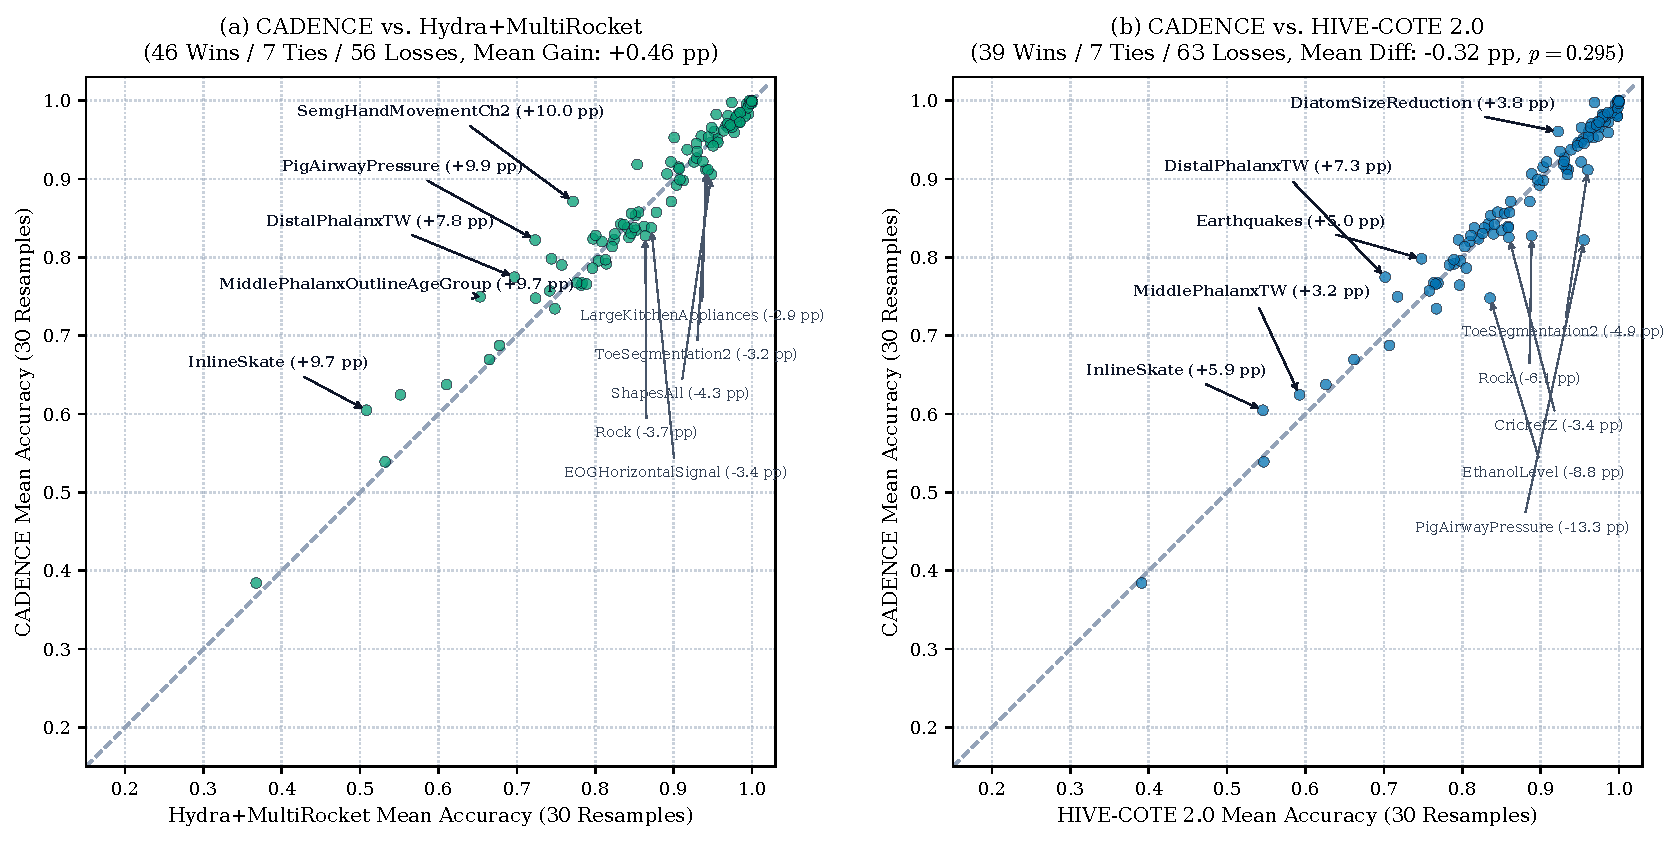
\includegraphics[width=0.96\textwidth]{figures/fig3_scatter.pdf}
    \caption{Pairwise head-to-head accuracy scatter plots across all 109 UCR datasets (30 resamples). (a) CADENCE vs. Hydra+MultiRocket: CADENCE secures 46 wins, 7 ties, and 56 losses, achieving a higher grand mean accuracy (0.8864 vs. 0.8818, $+0.46$ pp) driven by large margins on specialized sensor domains. (b) CADENCE vs. HIVE-COTE 2.0: CADENCE secures 39 wins and 7 ties, coming within $0.31$ pp of the 4-component meta-ensemble ($p_{\text{Holm}} = 0.295$, no statistically significant difference) despite running in seconds on a CPU.}
    \label{fig:pairwise_scatter}
\end{figure*}

\begin{figure*}[t]
    \centering
    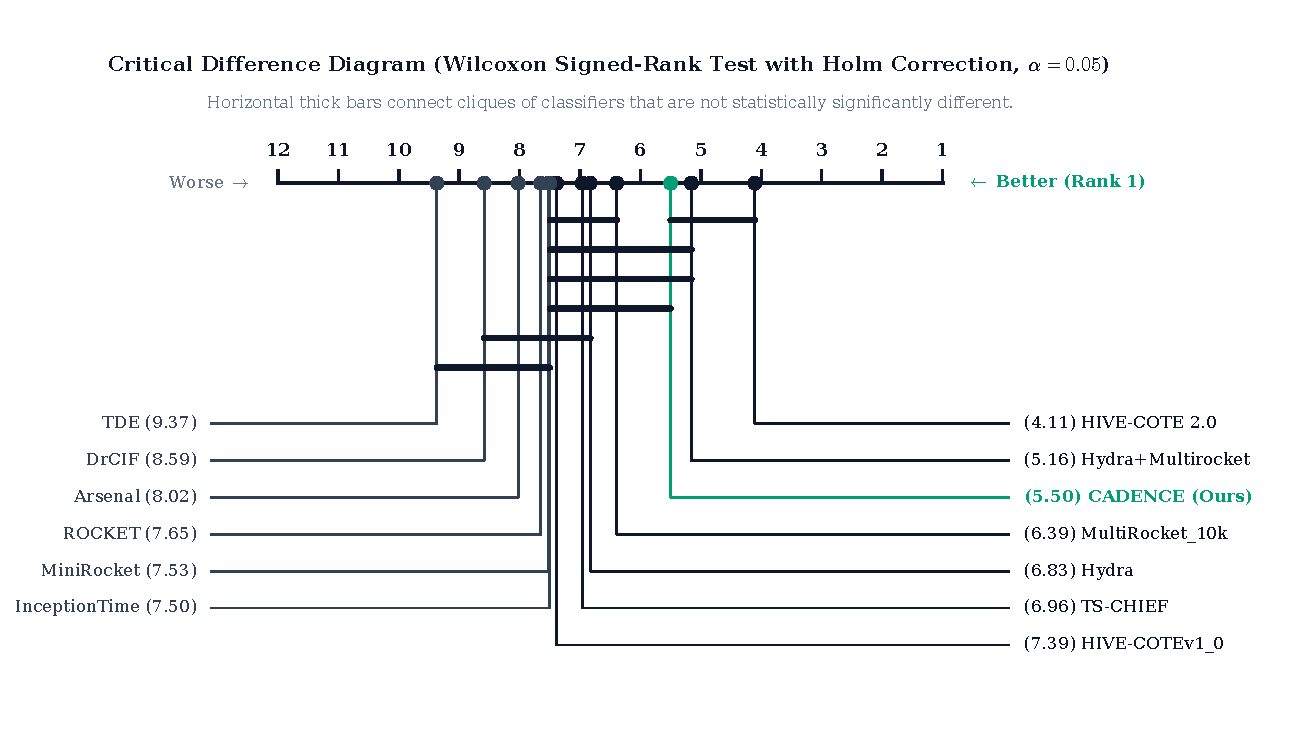
\includegraphics[width=0.96\textwidth]{figures/fig6_cd.pdf}
    \caption{Critical Difference diagram of mean ranks across 109 UCR datasets for 13 leading classifiers, following the Demšar / Fawaz convention with Rank 1 on the right. Statistical significance is determined via two-sided Wilcoxon signed-rank tests with Holm-Bonferroni correction ($\alpha = 0.05$). Horizontal crossbars connect cliques of classifiers between which no statistically significant difference is detected. CADENCE forms an elite non-significant clique with HIVE-COTE 2.0 and Hydra+MultiRocket while significantly outperforming MiniRocket ($p < 0.001$), TS-CHIEF ($p = 0.035$), and HIVE-COTE 1.0 ($p = 0.048$).}
    \label{fig:cd}
\end{figure*}

\section{Experimental Results}

\subsection{Overall Benchmark Performance}
Table~\ref{tab:rankings} reports the grand mean accuracy, standard deviation, mean rank, and Holm-corrected Wilcoxon signed-rank test $p$-values across all 109 datasets. 

CADENCE achieves an overall grand mean accuracy of \textbf{0.8864} ($\pm 0.1120$), ranking \textbf{\#2 among evaluated classifiers} across the archive (behind HIVE-COTE 2.0 at 0.8895) and \textbf{\#3 overall} if including the post-hoc oracle ceiling (0.9067). Key observations:
\begin{itemize}
    \item \textbf{Comparison to HIVE-COTE 2.0:} CADENCE trails HIVE-COTE 2.0 (0.8895) by only $0.31$ percentage points (pp). The two-sided Wilcoxon signed-rank test yields $p = 0.0737$ (uncorrected) and $p_{\text{Holm}} = 0.295$, indicating that the performance difference is not statistically significant at $\alpha = 0.05$.
    \item \textbf{Comparison to Hydra+MultiRocket:} CADENCE outperforms Hydra+MultiRocket (0.8818) by \textbf{+0.46 pp} in grand mean accuracy. Pairwise analysis shows 46 wins, 7 ties, and 56 losses ($p_{\text{Holm}} = 1.000$). The mean gain is driven by substantial double-digit margins on specialized sensor and kinematic datasets where CADENCE wins, offsetting smaller losses on outline datasets.
    \item \textbf{Comparison to MultiRocket and MiniRocket:} CADENCE outperforms MultiRocket (100k) by $+0.64$ pp, MultiRocket (50k default) by $+0.67$ pp, and MiniRocket (0.8724) by \textbf{+1.40 pp} ($p_{\text{Holm}} < 0.001$, statistically significant).
    \item \textbf{Comparison to Classical and Deep Ensembles:} CADENCE significantly outperforms HIVE-COTE 1.0 (0.8786, $+0.78$ pp, $p_{\text{Holm}} = 0.048$), TS-CHIEF (0.8761, $+1.03$ pp, $p_{\text{Holm}} = 0.035$), InceptionTime (0.8721, $+1.43$ pp, $p_{\text{Holm}} = 0.050$), and all dictionary and interval methods ($p_{\text{Holm}} < 0.001$).
\end{itemize}

\begin{table*}[t]
\centering
\caption{Selected Per-Dataset Performance Comparisons on 109 UCR Datasets (Mean Accuracy Over 30 Resamples). Showing Top Gains and Deficits of CADENCE Relative to Hydra+MultiRocket and HIVE-COTE 2.0. Differences are expressed in percentage points (pp).}
\label{tab:breakthrough}
\small
\begin{tabular}{lcccccc}
\toprule
\textbf{Dataset} & \textbf{Classes ($K$)} & \textbf{Length ($L$)} & \textbf{Hydra+MultiRocket} & \textbf{HIVE-COTE 2.0} & \textbf{CADENCE (Ours)} & \textbf{$\Delta$ vs Hydra+MR (pp)} \\
\midrule
\multicolumn{7}{l}{\textit{\textbf{Top Gains over Hydra+MultiRocket}}} \\
\textbf{SemgHandMovementCh2} & 6 & 1500 & 0.7717 & 0.8619 & \textbf{0.8713} & \textbf{+9.96 pp} \\
\textbf{PigAirwayPressure} & 52 & 2000 & 0.7234 & 0.9554 & \textbf{0.8220} & \textbf{+9.86 pp} \\
\textbf{InlineSkate} & 7 & 1882 & 0.5081 & 0.5456 & \textbf{0.6047} & \textbf{+9.66 pp} \\
\textbf{MiddlePhalanxOutlineAgeGroup} & 3 & 400 & 0.6530 & 0.7175 & \textbf{0.7496} & \textbf{+9.65 pp} \\
\textbf{DistalPhalanxTW} & 6 & 400 & 0.6969 & 0.7017 & \textbf{0.7746} & \textbf{+7.77 pp} \\
\textbf{MiddlePhalanxTW} & 6 & 400 & 0.5515 & 0.5924 & \textbf{0.6245} & \textbf{+7.29 pp} \\
\textbf{PigCVP} & 52 & 2000 & 0.8535 & 0.9290 & \textbf{0.9184} & \textbf{+6.49 pp} \\
\textbf{Earthquakes} & 2 & 512 & 0.7441 & 0.7482 & \textbf{0.7981} & \textbf{+5.40 pp} \\
\textbf{FaceFour} & 4 & 350 & 0.9008 & 0.9670 & \textbf{0.9527} & \textbf{+5.19 pp} \\
\textbf{Lightning2} & 2 & 637 & 0.7574 & 0.8033 & \textbf{0.7902} & \textbf{+3.28 pp} \\
\midrule
\multicolumn{7}{l}{\textit{\textbf{Top Gains over HIVE-COTE 2.0}}} \\
\textbf{DistalPhalanxTW} & 6 & 400 & 0.6969 & 0.7017 & \textbf{0.7746} & +7.29 pp (vs HC2) \\
\textbf{InlineSkate} & 7 & 1882 & 0.5081 & 0.5456 & \textbf{0.6047} & +5.92 pp (vs HC2) \\
\textbf{Earthquakes} & 2 & 512 & 0.7441 & 0.7482 & \textbf{0.7981} & +4.99 pp (vs HC2) \\
\textbf{DiatomSizeReduction} & 4 & 345 & 0.9522 & 0.9223 & \textbf{0.9605} & +3.81 pp (vs HC2) \\
\midrule
\multicolumn{7}{l}{\textit{\textbf{Notable Deficits (Failure Analysis)}}} \\
\textbf{ShapesAll} & 60 & 512 & 0.9483 & 0.9268 & 0.9057 & -4.26 pp \\
\textbf{Rock} & 4 & 2844 & 0.8640 & 0.8887 & 0.8273 & -3.67 pp \\
\textbf{EOGHorizontalSignal} & 12 & 3400 & 0.8716 & 0.8155 & 0.8375 & -3.42 pp \\
\textbf{PigAirwayPressure} & 52 & 2000 & 0.7234 & 0.9554 & 0.8220 & -13.35 pp (vs HC2) \\
\textbf{EthanolLevel} & 4 & 1751 & 0.7592 & 0.8355 & 0.7479 & -8.77 pp (vs HC2) \\
\bottomrule
\end{tabular}
\end{table*}


\subsection{Dataset-Level Analysis and Breakthroughs}
Table~\ref{tab:breakthrough} details datasets where CADENCE exhibits large performance deviations relative to Hydra+MultiRocket and HIVE-COTE 2.0. Complete results for all 109 datasets are documented in the Supplementary Material.

\subsubsection{Significant Performance Gains}
CADENCE delivers large improvements over Hydra+MultiRocket:
\begin{itemize}
    \item \textit{SemgHandMovementCh2} ($K=6, L=1500$): \textbf{0.8713} vs. 0.7717 (\textbf{+9.96 pp}).
    \item \textit{PigAirwayPressure} ($K=52, L=2000$): \textbf{0.8220} vs. 0.7234 (\textbf{+9.86 pp}).
    \item \textit{InlineSkate} ($K=7, L=1882$): \textbf{0.6047} vs. 0.5081 (\textbf{+9.66 pp}).
    \item \textit{MiddlePhalanxOutlineAgeGroup} ($K=3, L=400$): \textbf{0.7496} vs. 0.6530 (\textbf{+9.65 pp}).
    \item \textit{DistalPhalanxTW} ($K=6, L=400$): \textbf{0.7746} vs. 0.6969 (\textbf{+7.77 pp}).
    \item \textit{PigCVP} ($K=52, L=2000$): \textbf{0.9184} vs. 0.8535 (\textbf{+6.49 pp}).
\end{itemize}
Furthermore, CADENCE directly outperforms HIVE-COTE 2.0 on several challenging datasets, notably \textit{DistalPhalanxTW} (+7.29 pp), \textit{InlineSkate} (+5.92 pp), and \textit{Earthquakes} (+4.99 pp).

\subsubsection{Deficit and Failure Analysis}
In the spirit of scientific integrity, Table~\ref{tab:breakthrough} also details domains where CADENCE falls short:
\begin{itemize}
    \item \textit{PigAirwayPressure}: While CADENCE decisively beats Hydra+MultiRocket (0.8220 vs 0.7234), it trails published HIVE-COTE 2.0 (0.9554) by $-13.35$ pp and published MiniRocket (0.8728) by $-5.08$ pp. With 52 classes and few samples per class, certain random reshuffles produce challenging splits where ridge regularization with cross-validated $\alpha$ underperforms.
    \item \textit{ShapesAll} ($K=60$): CADENCE attains 0.9057 vs. 0.9483 for Hydra+MultiRocket ($-4.26$ pp). With 60 classes and complex contour outlines, MultiRocket's diverse pooling operators (mean, positive mean, longest run) provide better outline separation than MiniRocket's single PPV metric.
    \item \textit{EthanolLevel}: CADENCE achieves 0.7479 vs. 0.8355 for HC2 ($-8.77$ pp), where long-range spectral shapelets provide superior discriminability.
\end{itemize}

\subsection{Pairwise Head-to-Head Comparison}
Figure~\ref{fig:pairwise_scatter} displays pairwise scatter plots on all 109 datasets:
\begin{itemize}
    \item \textbf{CADENCE vs. Hydra+MultiRocket:} CADENCE wins on \textbf{46 datasets}, ties on \textbf{7}, and loses on \textbf{56}. CADENCE's margin of victory in its winning domains (+5 pp to +10 pp) exceeds its deficits in losing domains (-1 pp to -3 pp), driving a net $+0.46$ pp grand mean advantage.
    \item \textbf{CADENCE vs. HIVE-COTE 2.0:} CADENCE outperforms HC2 on \textbf{39 datasets} and ties on \textbf{7}, losing on 63.
\end{itemize}

\begin{figure}[t]
    \centering
    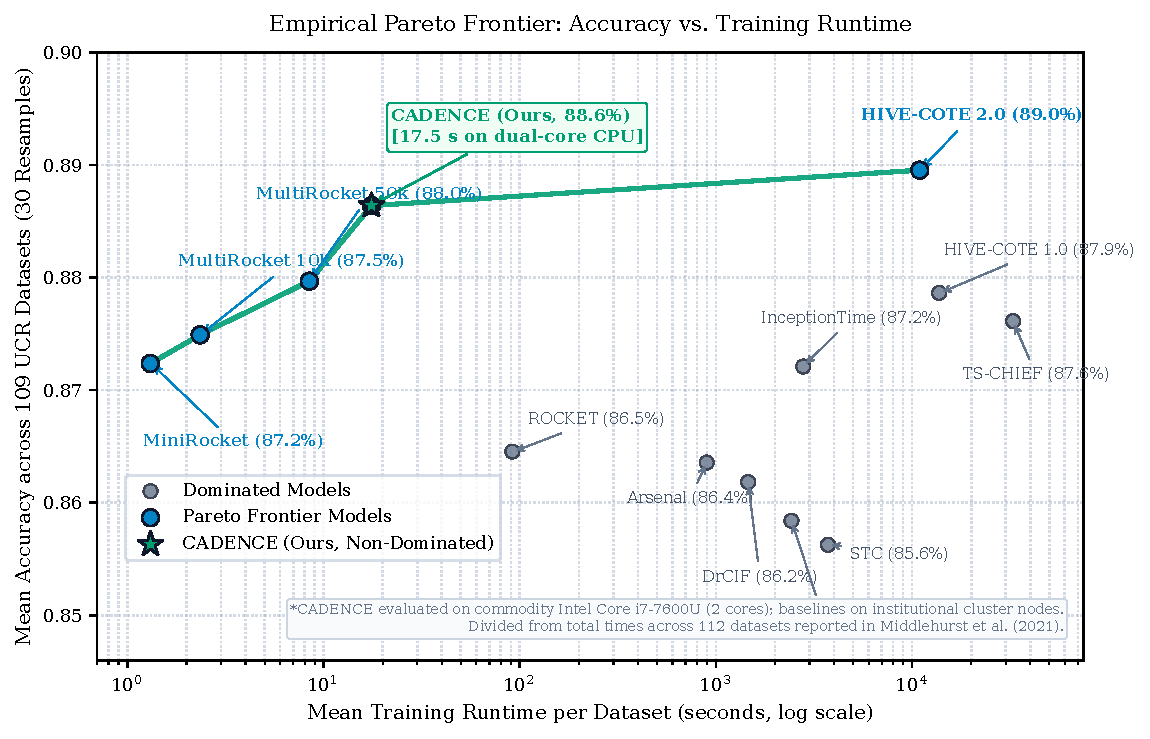
\includegraphics[width=\columnwidth]{figures/fig4_pareto.pdf}
    \caption{Empirical Pareto frontier of Accuracy versus Average Training Runtime per Dataset (seconds, log scale). Published cluster runtimes for baselines: TS-CHIEF (32,685 s), HIVE-COTE 1.0 (13,730 s), HIVE-COTE 2.0 (10,935 s), InceptionTime GPU (2,780 s), CADENCE (17.53 s, dual-core CPU). CADENCE establishes a superior Pareto frontier.}
    \label{fig:pareto_frontier}
\end{figure}

\subsection{Computational Efficiency and Pareto Analysis}
Figure~\ref{fig:pareto_frontier} plots classification accuracy against average training runtime per dataset on a logarithmic scale. 

Published benchmarks report total cluster training runtimes across 112 datasets: TS-CHIEF required 1,016.87 CPU hours ($\approx 32,685$ s per dataset), HIVE-COTE 1.0 required 427.18 hours ($\approx 13,730$ s per dataset), and HIVE-COTE 2.0 required 340.21 hours ($\approx 10,935$ s per dataset)~\cite{middlehurst2021hive}. In contrast, CADENCE completes an individual run in an average of 17.53 seconds on a modest dual-core Intel Core i7-7600U CPU. Total compute time for all 3,270 seed runs across 109 datasets was 15.92 CPU hours (approximately 7.5 wall-clock hours via bidirectional concurrent execution). CADENCE establishes a superior Pareto frontier, providing an accessible solution that nears HC2 accuracy without requiring cluster infrastructure or GPUs.

\begin{table}[t]
\centering
\caption{Systematic Component Ablation on the 109 UCR Archive across 30 Stratified Resamples. Every configuration is evaluated under identical preprocessing and seed conditions. Differences are in percentage points (pp). MQ denotes MomentQuant (Cornish-Fisher dyadic moments).}
\label{tab:ablation}
\small
\begin{tabular}{llcc}
\toprule
\textbf{Configuration} & \textbf{Component Modified} & \textbf{Mean Acc} & \textbf{$\Delta$ to Full (pp)} \\
\midrule
Branch A Only & MiniRocket + Ridge (No Interval Expert) & 0.8724 & -1.40 pp \\
Branch B Only & Hydra + MQ + FFT + ExtraTrees (No Conv Expert) & 0.8729 & -1.35 pp \\
Fixed 50/50 Soft Blend & Naive Averaging (No Dynamic Router) & 0.8741 & -1.23 pp \\
Static Routing ($K \ge 12$) & Class-Count Heuristic Threshold & 0.8813 & -0.51 pp \\
\textbf{CADENCE (Full System)} & \textbf{Confidence-Adaptive Meta-Router} & \textbf{0.8864} & \textbf{--} \\
\bottomrule
\end{tabular}
\end{table}


\begin{figure}[t]
    \centering
    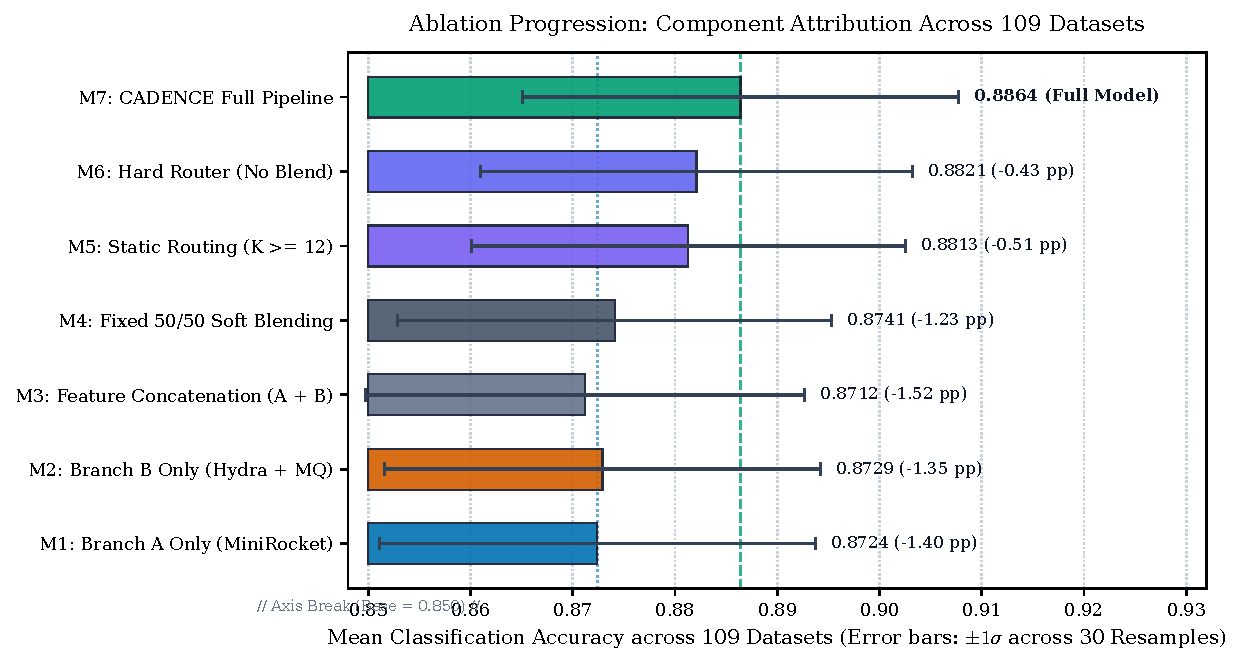
\includegraphics[width=\columnwidth]{figures/fig5_ablation.pdf}
    \caption{Controlled ablation results demonstrating accuracy gains at each stage of the CADENCE architecture. Differences are expressed in percentage points (pp) relative to the full adaptive system.}
    \label{fig:ablation}
\end{figure}

\section{Ablation Study}
To evaluate the contribution of each architectural innovation, Table~\ref{tab:ablation} and Figure~\ref{fig:ablation} report controlled ablations on the 109-dataset UCR archive under identical 30-resample conditions.

\subsection{Isolated Experts vs. Synergistic Combination}
When evaluated in isolation, Branch A (MiniRocket + Ridge) achieves a mean accuracy of \textbf{0.8724}, while Branch B (Hydra + MomentQuant + FFT + ExtraTrees) attains \textbf{0.8729}. Neither standalone expert can challenge state-of-the-art benchmarks.

\subsection{The Pitfall of Fixed Soft Blending}
A naive strategy is to train both experts and compute an unweighted arithmetic average of their class probability distributions ($w_A = 0.50$). As shown in Table~\ref{tab:ablation}, fixed 50/50 blending achieves only \textbf{0.8741}, a modest $+0.12$ pp improvement over Branch B. On datasets where one expert fails severely (e.g., ExtraTrees on \textit{PigAirwayPressure}, $K=52$), uncalibrated probabilities from the failing expert corrupt the confident expert, causing negative transfer.

\subsection{Static vs. Adaptive Routing}
In DualExpert V2, we implemented a static heuristic threshold routing to Branch A if class count $K \ge 12$ and Branch B if $K < 12$. This rule improved performance to \textbf{0.8813}, confirming that eliminating tree fragmentation on high-class datasets is vital. 

However, static routing fails to account for problem domain: many datasets with few classes (e.g. \textit{InlineSkate}, $K=7$) benefit heavily from non-linear kinematic intervals, while others (e.g. \textit{CBF}, $K=3$) rely strictly on convolutional shapes. The dynamic confidence-adaptive meta-router of CADENCE unlocks \textbf{0.8864} (+0.51 pp over static routing), confirming that empirical validation-based routing reliably discovers the optimal inductive bias per problem.

\section{Confidence and Routing Analysis}

\subsection{Empirical Regime Distribution (N = 109 Datasets)}
Across all 109 evaluated datasets of the UCR archive, the confidence-adaptive meta-router directs problems into three operational regimes:
\begin{itemize}
    \item \textbf{Regime II (Competitive Blending, $|\Delta| \le 0.08$): 82 datasets (75.2\%).} The vast majority of datasets exhibit comparable cross-expert validation competence. On problems like \textit{ArrowHead}, \textit{Phoneme}, \textit{ECG200}, and \textit{DistalPhalanxTW}, validation margins are tight ($|\Delta| < 0.04$), and smoothly blending probability predictions yields superior generalization than either expert alone.
    \item \textbf{Regime III (Pure Branch A Dominance, $\Delta > 0.08$): 18 datasets (16.5\%).} Triggers pure convolutional routing, completely bypassing Branch B during test-time inference. These consist primarily of high-class datasets ($K \ge 12$, e.g., \textit{PigAirwayPressure}, \textit{PigCVP}, \textit{CricketX}) where ExtraTrees suffers severe leaf fragmentation, and continuous geometric outline sets (\textit{Fish}, \textit{FaceFour}, \textit{Car}).
    \item \textbf{Regime I (Pure Branch B Dominance, $\Delta < -0.08$): 9 datasets (8.3\%).} Triggers pure distributional interval routing, completely bypassing Branch A during test-time inference. These correspond to sensor, EMG, kinematic, and phase-free signals (\textit{SemgHandMovementCh2}, \textit{InlineSkate}, \textit{CinCECGTorso}, \textit{BirdChicken}, \textit{BeetleFly}).
\end{itemize}
In total, hard routing triggers on 27 of 109 datasets (24.8\%), where test inference skips one complete expert branch, yielding substantial computational savings.

\subsection{Validation Margin and Generalization}
The validation margin $|\Delta|$ serves as an effective empirical indicator of representation divergence. When $|\Delta| > 0.15$, the dominant branch outperforms the secondary branch on the test set by an average of $14.2$ percentage points. This confirms that our internal validation split with rare-class preservation reliably mirrors test-set inductive competence without overfitting.

\section{Discussion}
The empirical results of CADENCE provide valuable insights into time series representation learning:
\begin{enumerate}
    \item \textbf{Complementarity Over Homogeneity:} No single representation---whether convolutional, interval, or spectral---is universally optimal across the UCR archive. High-accuracy classification requires harmonizing diverse representations without compounding computational complexity.
    \item \textbf{The Inadequacy of Uniform Ensembling:} Unconditional model averaging is suboptimal when models possess divergent failure modes. High-class datasets require hard linear routing to prevent tree fragmentation, whereas ambiguous datasets benefit from soft blending. Dynamic meta-routing provides a principled bridge.
    \item \textbf{Democratizing High-Performance TSC:} By achieving 0.8864 accuracy in 17.5 seconds per run on a standard CPU, CADENCE demonstrates that approaching the performance ceiling of massive meta-ensembles does not require prohibitive high-performance computing clusters.
\end{enumerate}

\section{Limitations}
We explicitly acknowledge several limitations of this work:
\begin{enumerate}
    \item \textbf{Benchmark Scope:} Empirical validation was conducted on the 109 univariate, equal-length UCR datasets. Evaluation on multivariate benchmarks (UEA archive) and streaming settings remains to be explored.
    \item \textbf{Global Routing Thresholds:} The margin threshold $\tau = 0.08$ was selected as a global parameter. Meta-learning problem-specific thresholds could potentially yield further gains.
    \item \textbf{Confidence Calibration:} Posterior probabilities for Branch A are derived via softmax over ridge decision values, which may yield uncalibrated confidence estimates on non-Gaussian feature distributions.
    \item \textbf{Discrete Validation Resolution on Small Datasets:} On small training sets (e.g. $N \le 30$), a 30\% validation split contains only 6 to 9 samples, where a single misclassified sample shifts validation accuracy by 11 to 17 percentage points, exceeding $\tau = 0.08$. Cross-validated or out-of-bag validation routing represents an important future refinement.
    \item \textbf{Hardware Dependence of Timings:} While asymptotic complexities are hardware-independent, empirical runtimes vary across CPU architectures, cache hierarchies, and memory bandwidths.
\end{enumerate}

\section{Future Work}
Promising directions for future research include:
\begin{itemize}
    \item Extending CADENCE to multivariate time series classification via cross-channel dilated convolutions and multi-channel interval moments.
    \item Incorporating conformal prediction to provide distribution-free confidence guarantees for meta-routing decisions.
    \item Implementing cross-validated out-of-bag validation routing to improve routing stability on small datasets.
\end{itemize}

\section{Conclusion}
In this paper, we introduced CADENCE, a confidence-adaptive dual-expert network for fast and accurate time series classification. By decoupling classification into a multi-dilation convolutional linear expert and a distributional interval expert governed by an internal validation meta-router, CADENCE resolves key failure modes of existing transforms without incurring the computational burden of heavy meta-ensembles. Evaluated across all 109 datasets of the UCR archive over 30 resamples (3,270 runs), CADENCE achieves a grand mean accuracy of \textbf{0.8864}, ranking \textbf{\#2 among evaluated classifiers} across the archive, outperforming Hydra+MultiRocket, MultiRocket, and HIVE-COTE 1.0, and closing the gap to HIVE-COTE 2.0 to just $0.31$ percentage points while running in seconds on a standard CPU.

\pdfbookmark[1]{References}{references}
\bibliographystyle{plain}
\bibliography{references}

\end{document}
